%% For double-blind review submission, w/o CCS and ACM Reference (max submission space)
% \documentclass[sigplan,10pt,review,anonymous]{acmart}\settopmatter{printfolios=true,printccs=false,printacmref=false}
%% For double-blind review submission, w/ CCS and ACM Reference
%\documentclass[acmsmall,review,anonymous]{acmart}\settopmatter{printfolios=true}
%% For single-blind review submission, w/o CCS and ACM Reference (max submission space)
%\documentclass[acmsmall,review]{acmart}\settopmatter{printfolios=true,printccs=false,printacmref=false}
%% For single-blind review submission, w/ CCS and ACM Reference
%\documentclass[acmsmall,review]{acmart}\settopmatter{printfolios=true}
%% For final camera-ready submission, w/ required CCS and ACM Reference
\documentclass[acmsmall,nonacm]{acmart}\settopmatter{}


%% Journal information
%% Supplied to authors by publisher for camera-ready submission;
%% use defaults for review submission.
\acmJournal{PACMPL}
\acmVolume{1}
\acmNumber{CONF} % CONF = POPL or ICFP or OOPSLA
\acmArticle{1}
\acmYear{2018}
\acmMonth{1}
\acmDOI{} % \acmDOI{10.1145/nnnnnnn.nnnnnnn}
\startPage{1}

%% Copyright information
%% Supplied to authors (based on authors' rights management selection;
%% see authors.acm.org) by publisher for camera-ready submission;
%% use 'none' for review submission.
\setcopyright{none}
%\setcopyright{acmcopyright}
%\setcopyright{acmlicensed}
%\setcopyright{rightsretained}
%\copyrightyear{2018}           %% If different from \acmYear

%% Bibliography style
\bibliographystyle{ACM-Reference-Format}
%% Citation style
%% Note: author/year citations are required for papers published as an
%% issue of PACMPL.
% \citestyle{acmauthoryear}   %% For author/year citations


%%%%%%%%%%%%%%%%%%%%%%%%%%%%%%%%%%%%%%%%%%%%%%%%%%%%%%%%%%%%%%%%%%%%%%
%% Note: Authors migrating a paper from PACMPL format to traditional
%% SIGPLAN proceedings format must update the '\documentclass' and
%% topmatter commands above; see 'acmart-sigplanproc-template.tex'.
%%%%%%%%%%%%%%%%%%%%%%%%%%%%%%%%%%%%%%%%%%%%%%%%%%%%%%%%%%%%%%%%%%%%%%


%% Some recommended packages.
\usepackage{booktabs}   %% For formal tables:
                        %% http://ctan.org/pkg/booktabs
\usepackage{subcaption} %% For complex figures with subfigures/subcaptions
                        %% http://ctan.org/pkg/subcaption
\usepackage{xcolor}
\usepackage{listings}
\lstset{
  basicstyle=\fontsize{8}{10}\selectfont\ttfamily,
  numbers=left,
  numberstyle= \tiny,
  keywordstyle= \color{ blue!70},
  commentstyle= \color{red!50!green!50!blue!50},
  frame=single,
  rulesepcolor= \color{ red!20!green!20!blue!20} ,
  escapeinside=``,
  xleftmargin=1.5em,xrightmargin=0em, aboveskip=1em,
  framexleftmargin=2em,
  showstringspaces=false,
  showtabs=false,
  breaklines=true
}
\lstdefinelanguage{Solidity}
{
  morekeywords={contract, mapping, address, uint, private, function, public, if, payable},
  morecomment=[l]{//},
  morestring=[b]"
}

% \usepackage{biblatex}

\usepackage{multicol}
\usepackage{lipsum}
\usepackage{mathtools}
\usepackage{cuted}

\usepackage{amsmath}
\usepackage{extpfeil}
\usepackage{mathpartir}
\usepackage[mathscr]{eucal}

\usepackage{caption}

\usepackage{hyperref}
\usepackage{cleveref}

% \usepackage[style=authoryear-comp]{biblatex}
% \DeclareLabeldate[online]{%
%   \field{date}
%   \field{year}
%   \field{eventdate}
%   \field{origdate}
%   \field{urldate}
% }
% \DeclareLabeldate{\field{date}\field{eventdate} \field{origdate}\literal{nodate}}

% \DefineBibliographyStrings{english}{%
% nodate = {\ifboolexpr{test{\ifentrytype{misc1}} or test{\ifentrytype{misc5}}}{}{o\adddot D\adddot}},
% }

\crefformat{section}{\S#2#1#3} % see manual of cleveref, section 8.2.1
\crefformat{subsection}{\S#2#1#3}
\crefformat{subsubsection}{\S#2#1#3}


\begin{document}

%% Title information
\title[Task-Specific Network Fusion through CDRP Model Decomposition and Assembly]{CS222 Project Proposal: Task-Specific Network Fusion through CDRP Model Decomposition and Assembly}         %% [Short Title] is optional;
%% when present, will be used in
%% header instead of Full Title.

\author{Zhongye Wang}
% \authornote{Student Number: 517030910353, Parallel Authorship}
% \authornote{Supervised by Qinxiang Cao, Shanghai Jiao Tong University, John Hopcroft Center for Computer Science.}          %% \authornote is optional;
%% can be repeated if necessary
%\orcid{nnnn-nnnn-nnnn-nnnn}             %% \orcid is optional
\affiliation{
	%\position{Position2b}
	%\department{Department2b}             %% \department is recommended
	\institution{Shanghai Jiao Tong University, 517030910353}           %% \institution is required
	%\streetaddress{Street3b Address2b}
	%\city{City2b}
	%\state{State2b}
	%\postcode{Post-Code2b}
	%\country{Country2b}                   %% \country is recommended
}
% \email{wangzhongye1110@sjtu.edu.cn}          %% \email is recommended

\author{Yichen Xie}
% \authornote{Student Number: 517030910355, Parallel Authorship}
% \authornote{Supervised by Qinxiang Cao, Shanghai Jiao Tong University, John Hopcroft Center for Computer Science.}          %% \authornote is optional;
%% can be repeated if necessary
%\orcid{nnnn-nnnn-nnnn-nnnn}             %% \orcid is optional
\affiliation{
	%\position{Position2b}
	%\department{Department2b}             %% \department is recommended
	\institution{Shanghai Jiao Tong University, 517030910355}           %% \institution is required
	%\streetaddress{Street3b Address2b}
	%\city{City2b}
	%\state{State2b}
	%\postcode{Post-Code2b}
	%\country{Country2b}                   %% \country is recommended
}
% \email{}          %% \email is recommended

\author{Xinyu Zhan}
% \authornote{Student Number: 517030910358, Parallel Authorship}
% \authornote{Supervised by Qinxiang Cao, Shanghai Jiao Tong University, John Hopcroft Center for Computer Science.}          %% \authornote is optional;
%% can be repeated if necessary
%\orcid{nnnn-nnnn-nnnn-nnnn}             %% \orcid is optional
\affiliation{
	%\position{Position2b}
	%\department{Department2b}             %% \department is recommended
	\institution{Shanghai Jiao Tong University, 517030910358}           %% \institution is required
	%\streetaddress{Street3b Address2b}
	%\city{City2b}
	%\state{State2b}
	%\postcode{Post-Code2b}
	%\country{Country2b}                   %% \country is recommended
}
% \email{}          %% \email is recommended


% %% Abstract
% %% Note: \begin{abstract}...\end{abstract} environment must come
% %% before \maketitle command
% \begin{abstract}
% 	Text of abstract \ldots
% \end{abstract}


%% 2012 ACM Computing Classification System (CSS) concepts
%% Generate at 'http://dl.acm.org/ccs/ccs.cfm'.

%% End of generated code


%% Keywords
%% comma separated list
\keywords{}  %% \keywords are mandatory in final camera-ready submission


%% \maketitle
%% Note: \maketitle command must come after title commands, author
%% commands, abstract environment, Computing Classification System
%% environment and commands, and keywords command.
\maketitle

% xyc, until the last
\section{Introduction}
% Recent years have witnessed the rapid development of deep learning.
The development of deep learning has proved its great capability, and it will be more beneficial if we can plant deep learning models into edge devices like wearable devices.
However, the limited energy supply and computational capability of edge devices lead to constraints on the scale and complexity of deep neural networks.
The edge devices often need only to perform very specific tasks, whereas the pre-trained models deals with more general cases.
This makes it possible for us to develop task-specific and light-weighted models to meet various constraints of edge device.

Network fusion is a potential way to further improve the performance of network models with the advance of edge devices, where we could deploy many models through devices, let them perform inference in parallel, and retrieve and join the results \cite{fang2019teamnet}.
Nevertheless, this could cause redundant complexity across models, making it unable to fully utilize the capability of each edge devices.

In this project, we will seek for a decomposition and a combination of light-weight neural networks to substitute the original complex model while preserving its functionality.
Moreover, we want to satisfy some given tasks (a subset of the original domain) with the minimum model complexity, i.e., the combination should assemble only necessary parts for the task-specific model.
% With this new model, we will try to reduce the parameter number and computing consumption notably at the expense of acceptable accuracy decline compared to the original large model.

% xyc
\section{Problem Description}
\label{sec:problem-desc}
The problem of our interest can be divided into two stages: network decomposition and network assembly.

We first look into the assembly task.
Given a set of decomposed small networks, each covers the classification\footnote{We will take the image recognition (classification) task as the example throughout the project.} task of a subset of the dataset, we need to find a subset of those models for any given tasks.
Following problems reflect the complexity of the assembly task:\begin{itemize}
  \item There could exist overlapping functionalities among models, i.e., several models could cover the classification of the same subset of samples, in which case we want a careful selection of those produce the optimal performance.
  \item The given task could be comparably simpler than that of the original model. We need to determine wether a given reduced model can satisfy the requirement and how to further reduce its complexity.
\end{itemize}

Two natural questions follows the above assembly task: how to find the initial set of decomposed small networks, and how to determine the sample subsets they cover.
That is the network decomposition task we are interested in.
An intuitive way to achieve such decomposition is to arrange samples into subsets according to their labels, and train separate models for each class.
Nevertheless, this makes the assembly task trivial, because there exists no overlapping among decomposed models and the problem can be solved in linear time by incrementally selecting required classes.
It also requires extra training, and the complexity for the resulting model could still be very large.
It is challenging to find a fine-grained decomposition of an existing model and dataset.

% We mainly focus on the task to replace a large deep learning model with a set of small models with reduced complexity.
% Using too many small models can still result in tremendous amount of calculation in inference and affect models' performance in edge devices, so we limit the overall complexity of models as well.
% % Then, the total computational consumption can decrease definitely.
% As a result, edge device can profit from the lowered demand for computational consumption.
% % And these small models are independent from the original deep learning network at least in the inference phase.
% % Hence, they can process the data on the edge device without communication with the cloud or servers, which extend the application range of these device.

% There are many possible approaches in the design of small model system.
% \begin{itemize}
%   \item We could train small models each with specific tasks, which can be implemented with satisfying performance and simple network structure.
%   \item We could train small models each dealing with part of the dataset, which can be combined to handle all data points efficiently.
% \end{itemize}
% Our focus will be the former one, where we want each model to perform binary decisions in the context of classification and the union of these models should uniquely determine the category of any sample.

% TODO: still an embedding?
% A more high-level understanding of the problem is to consider small models as feature extractors that jointly produce an embedding for the data sample.
% We can also retrieve such embedding implicitly using neural networks, but we choose to achieve the optimal embedding explicitly by solving the search problem formulated in \cref{sec:formulation}.

% We will take the image recognition (classification) task as the example throughout the project.
% At present, boosting\cite{Schapire1989The} tends to be one possible solution.
% However, the weaker learners in these algorithm, which may be very simple classifiers, are so susceptible that the outcome is sensitive to noisy data and outliers.
% By contrast, thanks to the application of neural networks and more sophisticated combination methods, we will attempt to pursue a more robust and accurate model.

% wzy
\section{Problem Formulation}
\label{sec:formulation}
% There has not been much time for us to fully consider the optimal way of addressing the problem, but we do propose one possible formulation and some solution ideas in this section.

In this section, we propose the critical data routing path (CDRP) decomposition for the decomposition task and a formal formulation of the assembly task.

\subsection{CDRP Models and CDRP Based Clustering}
In the context of convolutional neural network, critical data routing path \cite{wang2018interpret} \cite{yu2018distilling} describes subsets of filters in all convolutional layers, whose activations are important to the correct classification of some samples.
Removing them could cause significant performance drop for those samples, while preserving them only, the model still has high chance to classifies some of those samples correctly.

Wang \textit{et al.} trains a set of gates to either suppress or preserve the activation of each filters for one given sample to decrease the model complexity but maintain the correctness classification of the samples.
The preserved filters becomes the CDRP for the sample, and we get an over-fine-grained model decomposition per sample.
Also, the CDRP can also be some feature representation of the sample under the context of the original model, i.e., similar samples sharing the similar features will have high probability of sharing the same CDRP.
Based on this conjecture, we propose the CDRP clustering to merge decomposed models and find the corresponding covering set.

After learning the gates for each sample, we encode the sample using corresponding weights $\Lambda$ assigned to each gate.
We then cluster samples in this $Lambda$-space, and for samples in the same cluster, we might use the CDRP model of its centroid to correctly classify those samples, assuming the number of clusters is adequate.
This is true because their CDRP models are similar to the one of the centroid since we are using this similarity to perform the clustering.

We will take the rounded centroid CDRP models as the initial set of decomposed models and take corresponding clusters as the sample subset.

\paragraph{Remark.}
\label{par:side-project}
If two samples of different class are assigned the same cluster, they will activate almost identical filters in the original model, causing it to label them as the same class.
This gives us a potential way to analyze why the model makes mistakes in an intuitive way.
If time allows, we might consider this as a side project.

\subsection{Network Fusion of CDRP Models}
However, the CDRP decomposition makes the assembly problem for a single CNN model trivial, because this results in the same situation of the trivial decomposition we proposed in \cref{sec:problem-desc}.
We now have disjoint cluster of samples, where samples in the same cluster shares the same label (same arguments as the \textit{remark}~\ref{par:side-project}).
To cover a given set of classes, we only need to cover the set of clusters belonging to those classes, i.e., a linear algorithm to incrementally include corresponding CDRP models.
There are no feasible solutions other than the optimal one.

But luckily, things become quite different for multiple networks, and the CDRP decomposition makes the fine-grained network fusion possible.
Let us consider a very general example in Figure~\ref{fig:fusion-example}, where we want to fuse two different networks of the the same task but trained on two different dataset.
If we only want to determine wether a sample has the orange label correctly, we have following options: $(D_2 \cap C_3) \cup (D_3 \cap C_2)$, $(D_2 \cap C_1^c) \cup (D_3 \cap C_1^c)$, $(D_1^c \cap C_3) \cup (D_1^c \cap C_2)$, where $D^c$ is the compliment classifier.
The resulting performance could vary among different configurations.

\begin{figure}[h]
  \centering
  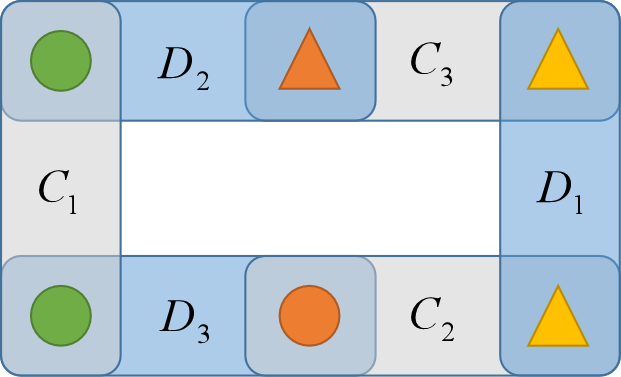
\includegraphics[width=0.38\linewidth]{fig/fusion_example.png}
  \caption{Joint CDRP Decomposition and Clustering on Two Dataset:
  We have a circle dataset and triangle dataset, where three colors represents three labels.
  The grey boxes are clusters from model $C$ trained on the circle dataset, and the blue ones are from model $D$ trained on the triangle dataset.}
  \label{fig:fusion-example}
\end{figure}

Such problem setting not only allow the problem to stay non-trivial, but also holds great significance in practice.
If we perform the clustering across datasets, we allow the fused model to generalize better and become more versatile.
Moreover, the fusion is more efficient, because we have removed many redundant feature overlapping in unit decomposed models.

\subsection{Assembling CDRP Models}
Next, we give a problem formulation that assembles the decomposed CRP models into a new model satisfying specific classification tasks.

Assume there are $N$ classes in total, each denoted by $A_i$.
We further divide each class $A_i$ into $M_i$ subsets $A_{ij}$ according to some features of samples, e.g., the activation of certain convolution filters.
Now, we have a set $\mathcal{D}$ of $K$ (a relatively large number) binary classifiers each identifying a subset of all $A_{ij}$ classes.
Say classifier $d$ separates $\{A_{ij} \,|\, (i, j) \in I_d\}$ from the rest of classes, i.e., given any sample, it determines wether the label of the sample belongs to $I_d$.
Here, $I_d$ is the positive label set defined by the classifier $d$.
Note that we can always define a compliment classifier whose positive label set is exactly the negative label set of the classifier $d$.

Given a target label set $\mathcal{A}$, our task is to find a subset $D^* \subset \mathcal{D}$, such that for any class $A_i \in \mathcal{A}$, there exists a partition that divides it into some subclasses $S_i^{(l)}$ where $A_i = \bigcup_l \{A_{ij} \,|\, (i, j) \in S_i^{(l)}\}$, and for each subclass $S_i^{(l)}$ there exists a subset of classifiers $D^{(l)} \subseteq D^*$ where $S_i^{(l)} = \bigcap_d \{I_d \,|\, d \in D^{(l)}\}$.
Here, subclass $S_i^{(l)}$ represents the union of some subsets $A_{ij}$ of class $A_i$, and the union of all subclasses of $A_i$ should reconstruct the $A_i$ itself.
The optimal set of classifiers $D^*$ should allow us to determine wether a sample belongs to any given subclass $S_i^{(l)}$ using a subset $D^{(l)}$ in it, which in turn determines wether the sample belongs to $A_i$.

\begin{figure}[h]
    \centering
    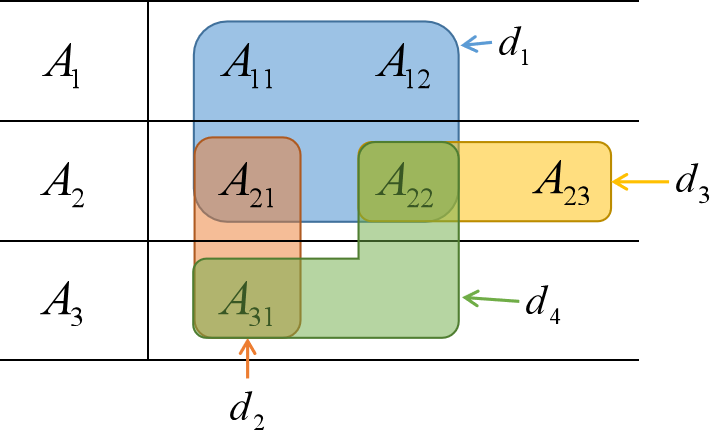
\includegraphics[width=0.45\linewidth]{fig/formulation_example.png}
    \caption{An Example Problem Setting:
    The samples in class $A_1$ is further divided into $A_{11}, A_{12}$ and those in class $A_2$ is further divided into $A_{21}, A_{22}, A_{23}$.
    We do not divide $A_3$ but rename it to $A_{31}$.
    There are 4 discriminators $d_1, d_2, d_3, d_4$ respectively identify $\{A_{11}, A_{12}, A_{21}, A_{22}\}$, $\{A_{21}, A_{31}\}$, $\{A_{22}, A_{23}\}$, and $\{A_{22}, A_{31}\}$.}
    \label{fig:feasible-example}
\end{figure}

Figure~\ref{fig:feasible-example} shows an example problem setting, and we give solutions to the following two instances of the problem:
\begin{itemize}
  \item \textbf{$\mathcal{A} = \{A_1, A_2, A_3\}$:}
  A feasible solution is $D = \{d_1, d_2, d_3\}$, which covers all classes because: \begin{enumerate}
    \item[\textit{(a)}] the intersection of $d_2, d_3$'s compliments identifies $A_1 = A_{11} \cup A_{12}$;
    \item[\textit{(b)}] the intersection of $d_1$ and $d_2$ identifies $A_{21}$, and its union with $d_3$ determines the entire $A_2$;
    \item[\textit{(c)}] the intersection of $d_3$ and the compliment of $d_1$ determines $A_3 = A_{31}$.
  \end{enumerate}
  \item \textbf{$\mathcal{A} = \{A_3\}$:}
  A feasible solution is $D = \{d_2, d_4\}$ because \begin{enumerate}
    \item[\textit{(a)}] the intersection of $d_2$ and $d_4$ uniquely identifies $A_{31} = A_3$;
    \item[\textit{(b)}] we do not need to include other discriminators to distinguish between $A_1$ and $A_2$, as long as it classifies them as \textit{not $A_3$}.
  \end{enumerate}
\end{itemize}

There are further constraints and considerations of the optimal discriminator set $D^*$.
\begin{itemize}
    \item \textbf{Number of Classifiers.} We need to choose adequate number of classifiers $|D^*|$ so that it covers all classes. But we prefer to use as less classifiers as possible to save computational consumptions.
    \item \textbf{Network Size.} The size of each classifier is limited. Large networks as classifiers improve accuracy but slow down inferences. Therefore, we will have penalty for large classifiers.
    \item \textbf{Overall Accuracy.} We know the accuracy of each classifier as a prior, but we need to derive the overall accuracy based on it. The $D^*$ should optimize the overall accuracy along with other goals.
\end{itemize}
These are factors we will consider in the later development and we are open for other suggestions.

% Beside these factors, there are other implementation issues about the solution to the problem.
% We have considered a given search space for small models, where the performance and functionality of each model is known as a prior.
% This allows us to concentrate on the search part of the solution.
% Nevertheless, we do not have such a prior in practice.
% Instead, we need to determine the next small model to be explored during the search, which we could formulate as a local search problem.

% zxy
\section{Related Work}
There have been other similar works trying to understand and prune the complexity of the CNN.
Zhou \textit{et al.} \cite{zhou2018interpreting} \cite{zhou2018revisiting} seek to understand the influence of certain filters on the accuracy wrt. some specific classes of samples by ablation and dissection.
Their work provides certain explanations of the outcome, but they do not explain how their technique can be utilize to improve or compress the model and it is only useful for network interpretation.
Yu \textit{et al.} \cite{yu2018distilling} attempt to produce task-specific models with reduced complexity through critical path distillation.
They identify critical paths through activation visualization for specific classes, which is more efficient than training gates to find them in our work.
But this means their critical path models are at the class level and these models can not interact with other external models through network fusion.

Qin \textit{et al.} propose the CAPTOR \cite{qin2019captor}, a framework for filter pruning also through clustering.
Different from our clustering method, they perform the clustering on filters with similar activation maximization visualization and prune similar filters to remove redundances.
We could also use this technique to remove redundances within a CDRP model.
Their pruning is again performed at the class level, while ours assembly is performed at the feature level, which is more fine-grained.

On the topic of network fusion, there are also many marvelous researches.
Du \textit{et al.} \cite{du2017fused} use multiple DNNs to refine the detections of a pedestrian detection generator and fuse these DNNs by fusing their outputs.
This type of output level fusion is coarse-grained, where redundant feature extractions may have occurred in DNNs.
On the opposite, Feichtenhofer\cite{feichtenhofer2016convolutional} proposed an extremely fine-grained fusion of multiple CNNs for video action recognition, where they carry out spatial fusion and temporal fusion on the layer level and achieves state-of-the-art results.
However, there are common problems of both work.
Their framework are task-specific and is difficult to apply their techniques in other domains.
And their works do not aim to reduce the network complexity during the fusion process.

% embedding
% As mentioned before, our approach resembles the embedding method, which is a common practice to address the curse of dimensionality, where we map data points into a subspace with reduced dimensionality and carry out the task in this space \cite{2016ml}.
% This can be accomplished with Multiple Dimension Scaling (MDS) \cite{cox2000multidimensional} or implicitly train an embedding in the hidden layers of a neural network.
% However, we explicitly search for an embedding by searching the optimal discriminator set, where each discriminator simulates one component in the embedding and we could directly obtain the category of some samples.
% It is also possible to consider more complex way of classifying using the embedding like adding another layer of network to perform the classification step, but we will stick to the current setting in the early stages of the development.

% ensemble
% A similar method that uses several weak learners to accomplish tasks is the ensemble method, which has been explored by many researchers. 
% Beriman\cite{BreimanBagging} proposed a method for generating multiple versions of a predictor by making bootstrap replicates of the learning set. 
% However, this method actually increased the amount of computation since it trained the learned repeatedly.
% Schapire\cite{Schapire1989The} proposed the boosting method to converting a weak learning algorithm into one that achieved arbitrarily high accuracy by combining a set of weak learners.
% This method was developed by Freund \textit{et al.}\cite{Freund1995A}, who proposed an adaptive version of the boost.
% Subsequent weak learners were tweaked in favor of those instances misclassified by previous classifiers. 
% Friedman \textit{et al.}\cite{FriedmanGreedy} proposed a new method called gradient boosting. 
% It performed additive optimization in functional space, which compensated for the weakness of weak classifiers in the light of the gradient of their loss function.
% We will consider to include their ideas to ensemble models in our discriminator set.

%% Acknowledgments

% Bibliography
% \bibliographystyle{acm}
% \bibliographystyle{unsrt}
\bibliography{../full_list.bib}


%% Appendix
%\appendix
%\section{Appendix}

%Text of appendix \ldots

\end{document}